% UPDATED BY MARCUS SCHAGERBERG, 2023
% CREATED BY WOLFGANG AHRENDT, 2021

\section{Tools}

% WRITTEN BY JAKOB WINDT, 2023
\subsection{Unity}
    The traffic simulation tool is built in a well-known game-engine called Unity. There are a few reason why it was chosen as the development platform for the project instead of a similar game-engine like Unreal Engine. To begin with, C\# is the main programming language supported by Unity, which some of the team members had previous experience with. Furthermore, C\# is a higher level language compared to C++, the main language of Unreal Engine, making it easier for the team members without experience to learn. Because of this, the time it took to begin programming in the early stages of the project was most likely shorter, compared to if Unreal Engine was chosen as the platform.

    Another reason would be that Unity comes with the Unity Asset Store, a marketplace for acquiring creator made assets. This feature is important because, for example, instead of having to create custom models for the vehicles, they could instead be purchased using the given budget. This saves a lot of time, that could be better spent on other parts of the project. One of the more notable purchased assets is Edy's Vehicle Physics that are used to rig vehicle models with realistic physics. Instead of having to develop custom vehicle physics for each model, the team could instead use the asset to quickly configure a model with physics.

    The final reason why Unity was chosen, is because of its flexible developing structure. The level of customization available inside the engine is a lot greater when comparing to Unreal Engine. However, because of this, Unity ends up being more unstable whereas Unreal is far more stable and robust. 

% WRITTEN BY JAKOB WINDT, 2023
\subsection{GitHub}
    A commonly used tool when developing software in larger groups is Git. Git is a free and open-source version control system that allows its users to collaborate in a efficient and easy way. 

    GitHub is an online software development platform that utilizes Git to store and track software projects. It allows for users to work in their own separate branches, and later merge those into the main repository. Before a team member could merge their new code to the main repository, the code would have to be reviewed by at least one other team member to ensure that the code was well commented, functional, and that it follow the C\# coding standard.

% WRITTEN BY JAKOB WINDT, 2023
\subsection{Trello}
    It was decided early on that the projects work flow should follow the SCRUM and Agile software development practices. Trello is a website that hosts scrum-boards in an user-friendly way. This allowed the team to keep track of what needs to be worked on in the project during the sprints. A sprint is a set time period when new tickets are made, and completed.

% WRITTEN BY JAKOB WINDT, 2023
\subsection{Balsamiq Wireframes}
    During the first stage of creating a UI, its important to start with a simple mock-up design. This is what the tool, Balsamiq Wireframes, is used for. The user can quickly design wire frames depicting how the UI will appear during different times in the program. This includes everything from buttons to pop-up menu's that might appear in the simulation tool.

%% WRITTEN BY JAKOB WINDT, 2023
\subsection{Third-Party Assets}
    Built into Unity is their asset store. Instead of creating everything from scratch, the team opted to purchase some assets. An asset can be anything from a 3D model to animation and scripts. The two main assets purchased for the project are Edy's Vehicle Physics and European Road Signs. Edy's Vehicle Physics is a package that includes a tool that allows its user to easily implement realistic vehicle physics into 3d models. This saves a substantial amount of time in the end because there would be no need to create custom physics attribute for each vehicle model. 

    As the name states, the European Road Signs assets include a plethora of street signs, as well as an editor to customize them. Without this asset, there would have been a need to create custom 3D models and texture, which no team member had previous experience with.

\section{Simulation Design and Implementation}

\subsection{ABM}

% WRITTEN BY HANNES KAULIO, 2023
\subsection{Road Generation}
    In order to achieve realistic roads with adequate curves, composite Bézier curves were used. The Bézier control points will shape the road and its characteristics. A number of parameter can be changed in the Bézier path to change the appearance. The position and sharpness of the turn can be modified by changing were the control points are placed in relation to each other. 
    \inlineimage{figures/method/road_generation/bezier_path_unity.png}{Composite Bézier path}{0.5}

    While the Bézier curves give a good ground level for the road implementation, it is hard to implement and build logic based on it since it is a continuous path. The Bézier logic and its control points was abstracted away with a node implementation placed on top of the Bézier path. A number of nodes called RoadNodes is placed along the Bézier path at a rate dependent on curve of the road. The nodes are all connected the its previous and its next node along the path. The goal of these nodes is to carry enough information to procedurally  build the road mesh as well as carry some logic needed for agents to navigate the environment.
    \inlineimage{figures/method/road_generation/roadnodes.png}{Visual representation of RoadNodes places along a Composite Bézier path}{0.5}

    By using the RoadNodes, generating the road mesh is possible. The mesh is procedurally generated by placing vertices at the RoadNode and along its normal line in both direction at a length equal to the width of a lane. If multiple lanes is wanted, vertices can be continually added in each normal direction for the lane amount. In addition to these, vertices are also placed below them to add thickness to the road. Triangles are then drawn between these vertices to create the mesh. To add the road material, sub meshes is created for each lane. The power of procedural generation is the ability to customize the roads different parameters. The width of the lanes, width of the lines, thickness of the road and number of lanes can all be changed for each road.

    \inlineimage{figures/method/road_generation/road_mesh_generation.png}{The vertices and triangles used to generate the one lane road mesh}{0.5}

    \inlineimage{figures/method/road_generation/road.png}{Road generated from its RoadNodes}{0.5}

    While the RoadNodes carry a lot of critical logic, it is lacking logic for driving along the different road lanes. This logic is added with another node that is placed along the road, the LaneNode. LaneNodes are placed at both sides of the normal line of each RoadNode at the middle of the lanes. These nodes are responsible for the road steering as well as notifying other agents if they are currently occupied by any agents.

    \inlineimage{figures/method/road_generation/lane_nodes.png}{Visual representation of RoadNodes(Red) and LaneNodes(Green)}{0.5}

\subsection{Intersection Generation}

\subsection{Navigation in intersections}

% WRITTEN BY HANNES KAULIO, 2023
\subsection{City Generation}
    To aid in simulating cities and larger areas, existing real life locations are generated from OSM data. The OSM data specify the latitude and longitude of every road and its path. Real life building data is also used to generate a representation of the buildings. The OSM file is parsed and the roads are generated with its specified characteristics. The speed limit, road type and if the road is lit is all considered when generating the road.  

% WRITTEN BY HANNES KAULIO, 2023
\subsection{Navigation}
    The basic navigational responsibility of each agent is the ability to follow the road lanes, avoid colliding into other agents, follow the traffic rules and being able to navigate to a given position.

    In order to follow the lanes, each agent follow the LaneNodes on the road. The LaneNodes store all the information needed to navigate the road. The position of the node, the agent that is currently on the node and special traffic rules the vehicles need to follow are stored on the node. Traffic signs such as stop sign are represented as a node and the traffic logic can be accessed by the agent when they encounter the node. 

    The agents steer towards a node that is a certain distance in front of the car. This distance is influenced by the current speed. By steering towards nodes that are in front of the agent, a smooth and reliable steering is achieved. Similarly to steering, breaking is accomplished by looking at nodes at a certain distance ahead. When a node with stop logic is found, the agent will break and stop before that node. This is done by looking for stop nodes at a distance ahead equal to the break distance of the agent. The agents also claim each node they are over so other agents can stop when the node at the break distance is claimed.                                          

    To enable the ability to navigate the roads, a weighted directed graph is created from the roads. The graph nodes are all the road endpoints and intersections and POIs. The edges between the nodes are weighted with a cost that is calculated as the distance * the speed limit. The agents navigate to a given end node by receiving a path of edges from the A* algorithm. When an agent doesn't have an active navigation path, it will be assigned path that will lead it to a given destination. The agent maps out the path and saves instructions for were to turn in each intersection that is passed when navigating to the destination.
    \inlineimage{figures/method/road_generation/navigation_graph.png}{Visual representation of a navigation graph}{0.5}

\section{Performance}

% WRITTEN BY JAKOB WINDT, 2023
\subsection{Quality vs Performance}
    An important aspect of software is how well it runs. Therefore, it was decided early on that the functionality to change the quality level of the simulation should exist. 

    %% Vehicle performance
    While testing the simulation during development, the most noticeable performance cost were the vehicles on the roads. This is because of the Edy's Vehicle Physics asset that simulates real-world physics to each vehicle in the network. To circumvent this issue, a vehicle performance mode was implemented. This performance mode would disable the EVP asset, and instead move the cars by offsetting their individual object transform. As a result, the performance cost of the vehicles would decrease, and allow for more cars in the road network.

%% Road building performance



\subsection{Performance Benchmarks}

% WRITTEN BY JAKOB WINDT, 2023
\subsection{Optimization} 
    When creating software of any kind, it's always important to make sure it's able to run smoothly. To allow the program to run well, optimizations had to be made. There are two areas in the simulation that are costly performance-wise: the vehicles on the roads and the roads themselves. To optimise the vehicles, as mentioned earlier, a performance mode was implemented. This allowed the simulation to skip calculating the physics for each vehicle. 

    Furthermore, since the simulation is in 3d, the details of the vehicle models had to be accounted for. A 3d model is created with vertices, which are points in a 3d dimensional space. Three of these points are used to construct a triangle, and the triangles in turn build the model. The amount of triangles in a model determines the overall detail of said model. To improve the performance of the simulation, the models that were chosen most contain a low count of triangle, usually less than 20,000. 

    For the road network, % TODO

\section{Graphics}

\subsection{Animations}

\subsection{Environment Materials and Textures}


\section{User Interface}

%% WRITTEN BY JAKOB WINDT, 2023
\subsection{Design}
    To allow the user to interact with the simulation, an user interface was made. The UI consists of two main parts: the start menu and the overlay. 

    The start menu contains three buttons, one to start the simulation, one to enter the settings menu, and one to exit the program. The settings menu allows the user to change the volume, quality mode, enable a fps counter, and enter full screen. 

    The overlay that is visible while the simulation runs is what allows the user to interact with the simulation itself. There are two main types of buttons: the camera buttons and the menu buttons. %% TODO

\subsection{Statistics}


% WRITTEN BY MARTIN BLOM, 2023
\section{Work flow}
    When developing any software larger than just a single use script, the amount of work and information can quickly grow beyond the level of ones own simultaneous comprehension. Therefore these kinds of projects require rigorous planning and strategizing to not get lost in all the different tasks and do them in a smooth and reasonable order, that allows for parallel continuous progress.

    To achieve this a strict work flow framework was developed, where the first step was to analyze the work load and disposable time. This included drafting a time plan for the whole time scope of the project \ref{fig:time-plan}. 

    \begin{figure}[H]
        \centering
        \fbox{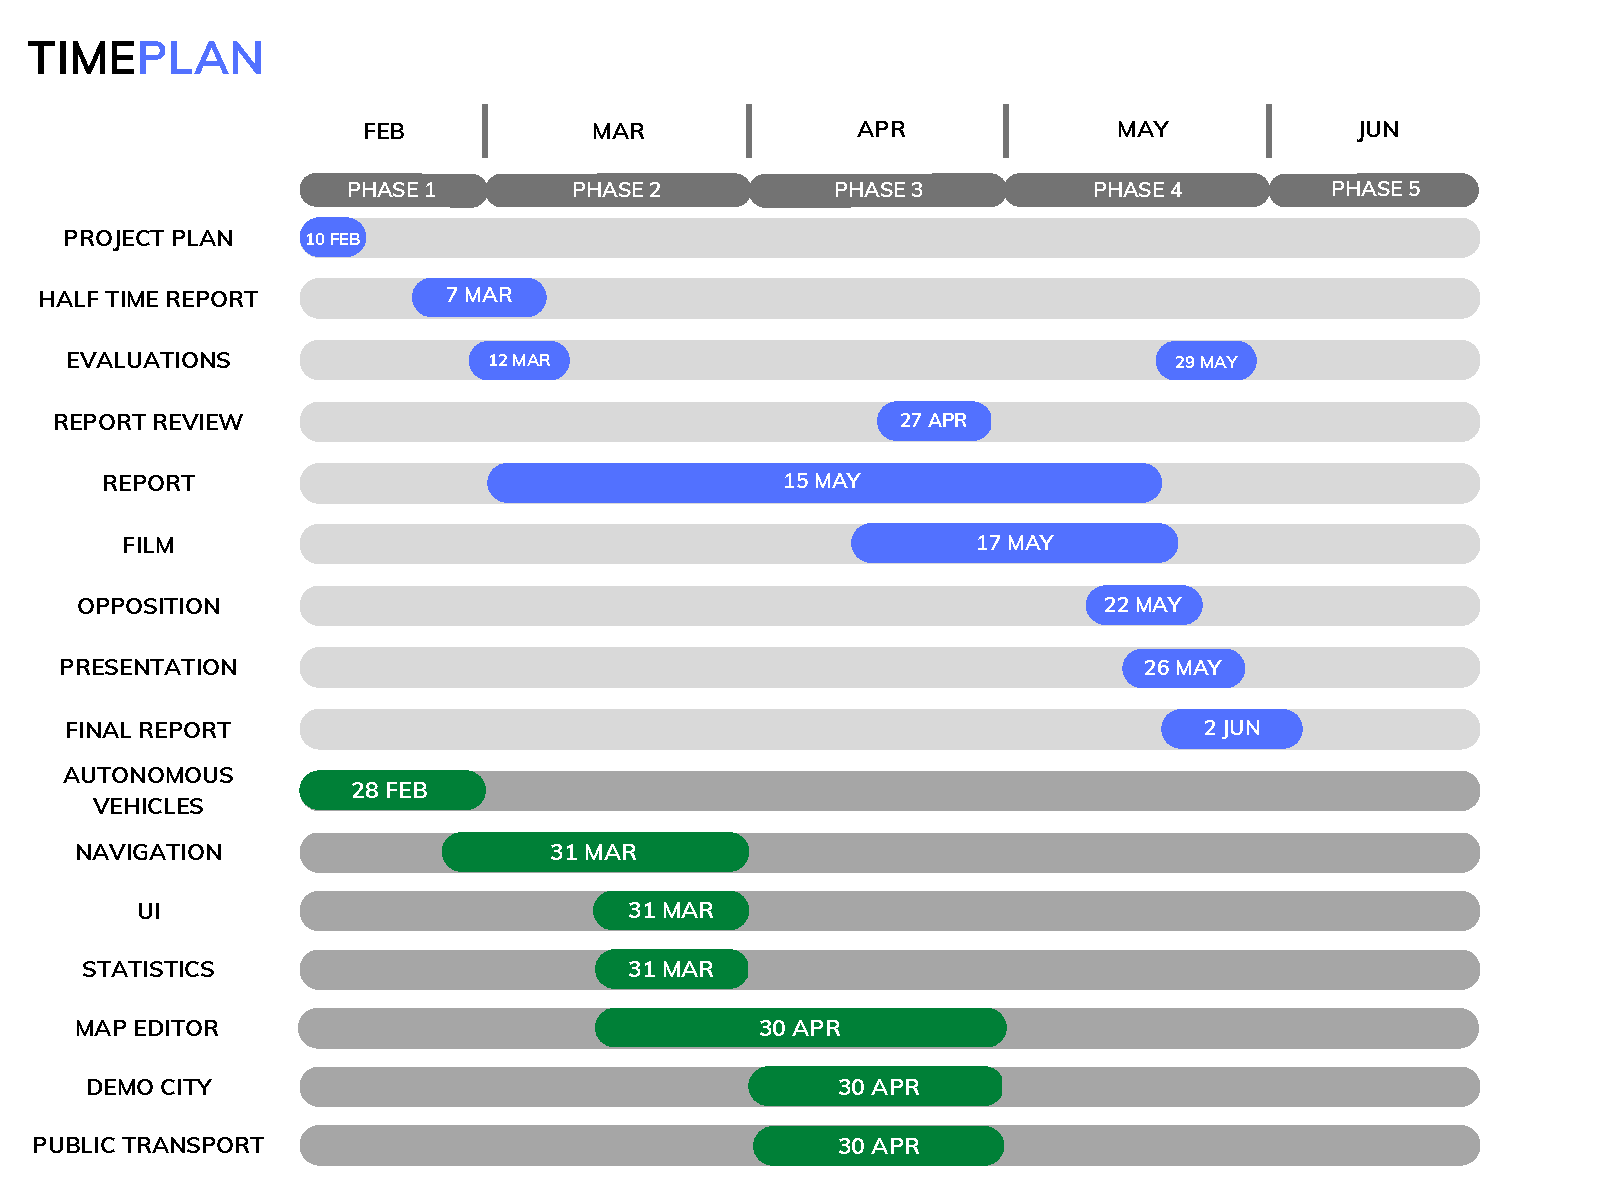
\includegraphics[scale=0.5]{Project_report/appendix/Time_plan.pdf}}
        \caption{Project Time Plan}
        \label{fig:time-plan}
    \end{figure}

    With this it's now much easier to keep track of the general progress of the project, as well as helping with planning short term goals. Coincidentally this is the next step of the work flow model. The short term goals where planned using a scrum framework with weekly sprints, explained in \ref{sub:weekly-sprints}. These sprints were upheld for the duration of the project to keep a stead flow of progress, together with the time plan they create a very clear way of seeing the current state of completeness. 

    The third aspect of the work flow is the approval of progress. As mentioned earlier a large project requires a substantial amount of planning to not get lost. The approval of progress can be seen as just as important as the planning and execution itself. Without a popper method of approving new advancements/functionality, the project can quickly falter. If progress never goes through the process of approval many things can go wrong. Evidently, badly written code can cause issues that are easily preventable with a quick inspection. Code can even be considered good but with no input from the rest of the team, visions of how higher order elements will be implemented can differ. This can implicitly create  more complex problems much further on, which can be very hard and time consuming to resolve. To solve this, code reviews \ref{sub:code-reviewing} for every change made are part of the workflow.  

\subsection{Weekly Sprints} \label{sub:weekly-sprints}
    The weekly sprint model stems from the scrum framework, which is a framework for developing and sustaining complex products. The sprint model follows 4 repeating stages of development: Planning, Implementation, Review and Retrospect.

    Each sprint starts out in the planning stage, where a meeting is held to set up this sprints goals. This includes moving/creating stories for the backlog as well as the current sprint. The stories are mainly chosen by the project manager then developed in unison with the scrum master and input from the rest of the team.

    The next stage of the sprint is the implementation itself. This is the time were the teams focus is solely on delivering good quality solutions to complete all of the current sprints stories, and eventually working on the backlog as time is presented.

    Next up is the review stage, not to be confused with code reviewing \ref{sub:code-reviewing}. In this stage another meeting is held called a "Demo meeting", where all members get to do a small demonstration of all their progress during the sprint. This is an important step to onboard all members on new functionality and make sure that desired behaviour is achieved. When a story is regarded as fully complete it's archived to make room for new ones.

    Lastly the retrospect stage, which is usually carried out following the review stage. In the retrospect stage the current sprints efficiency and quality is discussed. And plans/ways to increase these and the overall effectiveness are considered. When all is done the cycle begins anew until the project is done.

\subsection{Code Reviewing} \label{sub:code-reviewing}
    % TODO 
    % describe code review process

\section{Testing}